\documentclass{article}
\usepackage{graphicx} % Required for inserting images

\title{Homework 1 Bonus}
\author{Ayman Tawaalai}
\date{January 2024}

\begin{document}

\maketitle

\section{Introduction}
The purpose of this assignment is to conduct Exploratory Data Analysis (EDA) on 10 different data sets. These data sets are to be event sequences. Event sequences are recorded into the data set for an event that provides some context about the data set on a macro and micro level.
\section{Data Set 1}
The first data set EDA will be performed on is called "world\_population.csv" 
\begin{figure}
    \centering
    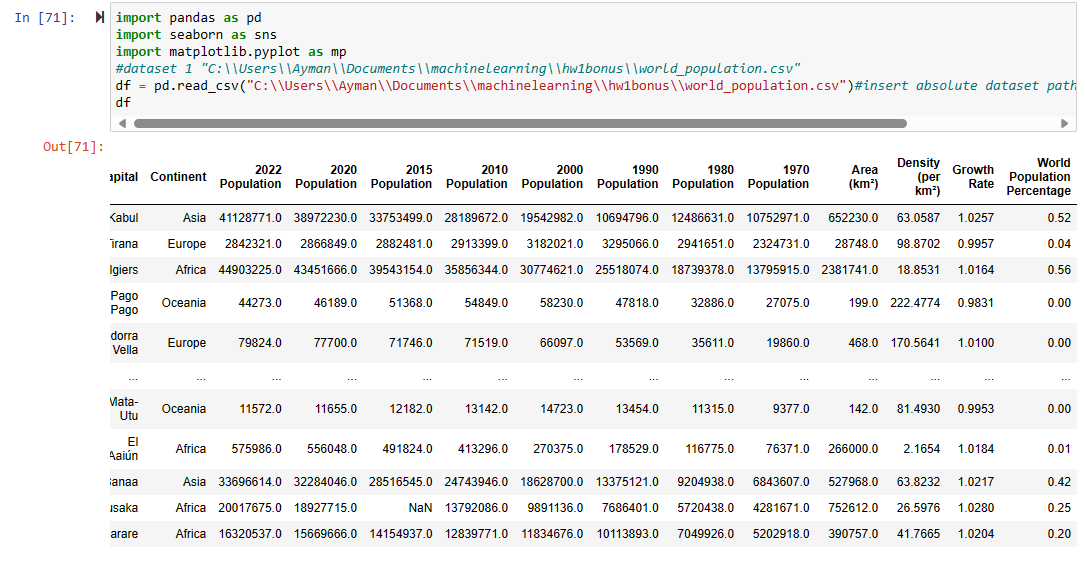
\includegraphics[width=0.5\linewidth]{image1.png}
    \caption{Data Frame of Data Set 1}
    \label{fig:enter-label}
\end{figure}
The data was pulled using a GitHub of "AlexTheAnalyst" and contains the population data of nations dating back to the year 1970. Additional information in the displayed data frame includes their growth rate, country density, size, and the population percentage in comparison to the rest of the world. 
\begin{figure}
    \centering
    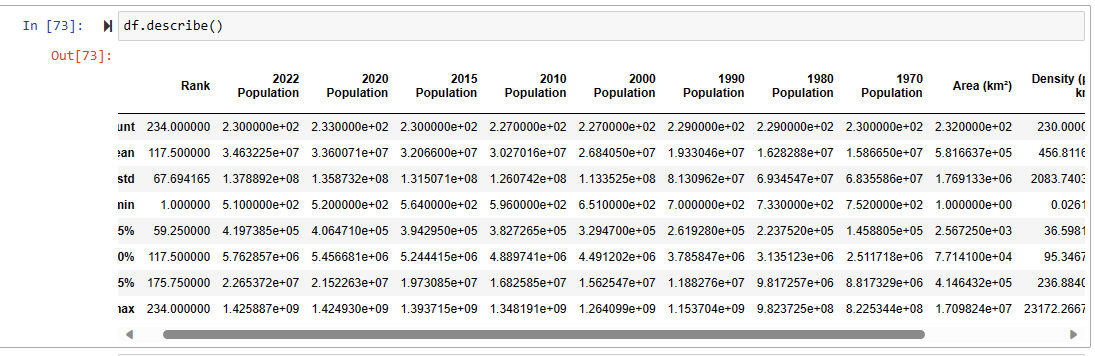
\includegraphics[width=0.5\linewidth]{image2.png}
    \caption{Data Frame Describe}
    \label{fig:enter-label}
\end{figure}
Figure 2 provides basic statistical information on the data set. An interesting piece of information is that the average growth rate is 1.01; this means that the average population is not increasing but meeting replacement levels of the previous generation. When searching for null values, the data set has many elements of null values. 
\begin{figure}
    \centering
    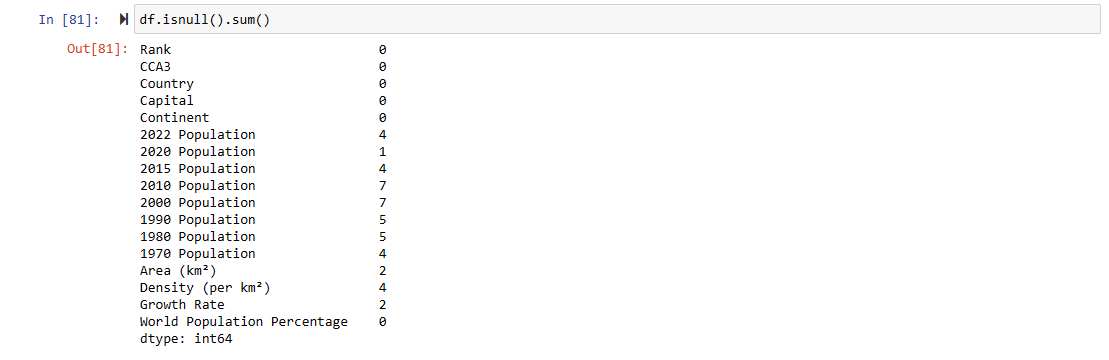
\includegraphics[width=0.5\linewidth]{image3.png}
    \caption{Data Frame nulls}
    \label{fig:enter-label}
\end{figure}
This information will be useful to ensure that during data clean up those values can be replaced with information from the basic statistical information and similarities. When searching for nations with the largest population percentage, China shows first throughout the years of data provided. Finally, when looking for correlation a heat map was used. The heat map shows that there is some correlation between a high population and the size of a country, however there are other instances where the correlation is not as clear because there will be areas of low density and high size.
\begin{figure}
    \centering
    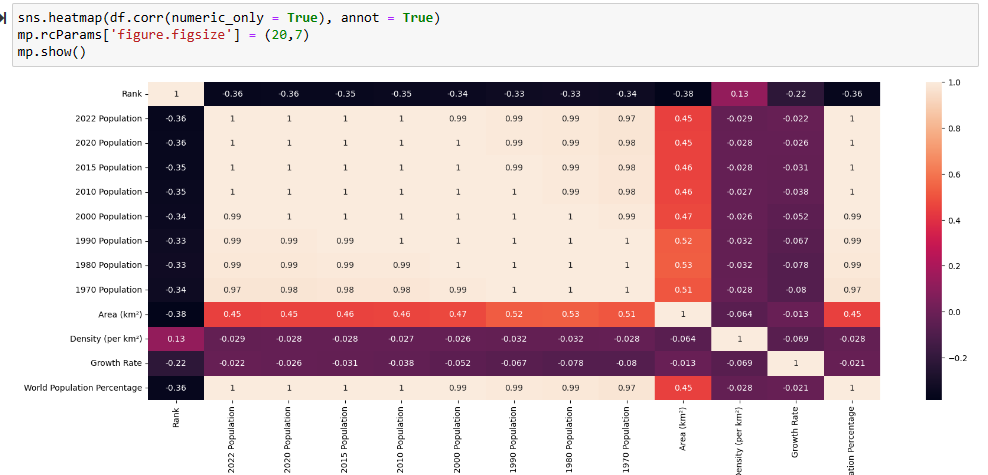
\includegraphics[width=0.5\linewidth]{image4.png}
    \caption{Data Frame Heat Map}
    \label{fig:enter-label}
\end{figure}
\section{Data Set 2}
The second data set EDA will be performed on is called "Online-Retail.csv". 
The data was pulled from the UC Irvine Machine Learning Repository. The data is about each product that was sold and on what invoice that product was on. Furthermore, additional information such as quantity, customer ID, and country of origin is present. When checking the data types, each item in the data frame will either be a float, int, or an object. 
\begin{figure}
    \centering
    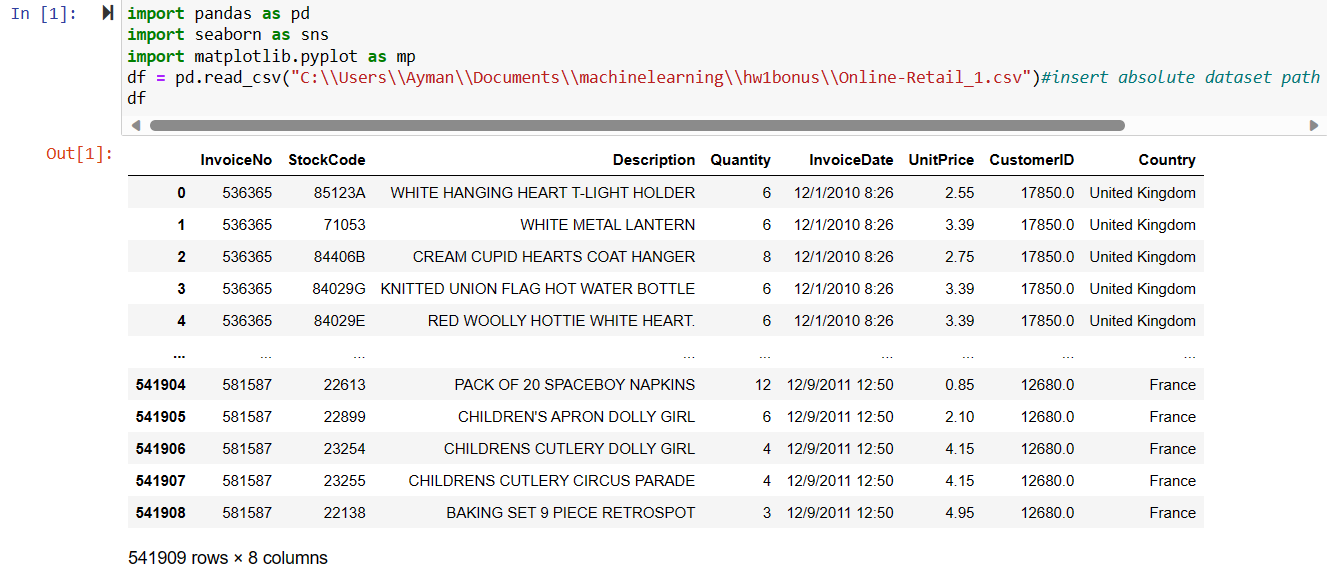
\includegraphics[width=0.5\linewidth]{a.png}
    \caption{Data Frame of Data Set 2}
    \label{fig:enter-label}
\end{figure}
When checking for null values, there are null values present in the description and customer ID. Although customer ID has null values, the stock code does not. What this means is that during clean up, one could look at the code and then search for the description using that code in a product database. 
\begin{figure}
    \centering
    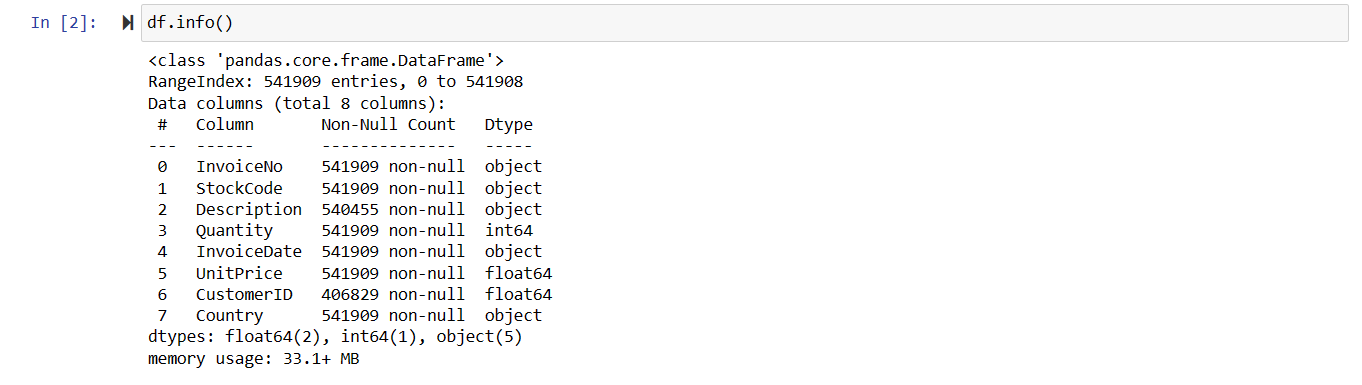
\includegraphics[width=0.5\linewidth]{b.png}
    \caption{Data Frame nulls}
    \label{fig:enter-label}
\end{figure}
When searching for which country has the most invoices the results show that it is unspecified. This means that although this can be interpreted as a "null value" since country data cannot be pulled or manipulated with.
\begin{figure}
    \centering
    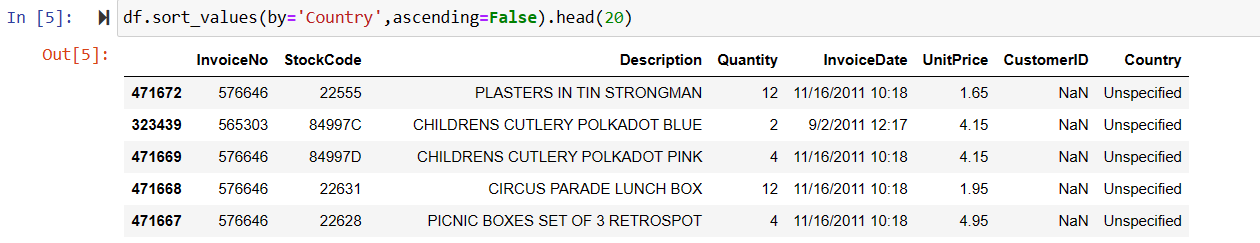
\includegraphics[width=0.5\linewidth]{c.png}
    \caption{Data Frame Max Country}
    \label{fig:enter-label}
\end{figure}

\section{Data Set 3}
The third data set EDA will be performed on is called "AirQualityUCI.csv". 
The data was pulled from the UC Irvine Machine Learning Repository. The data set holds the measure of air quality within an unspecified Italian city from March 2004 to February 2005. Air quality is measured hourly through different categorical means outlined in the data frame.
\begin{figure}
    \centering
    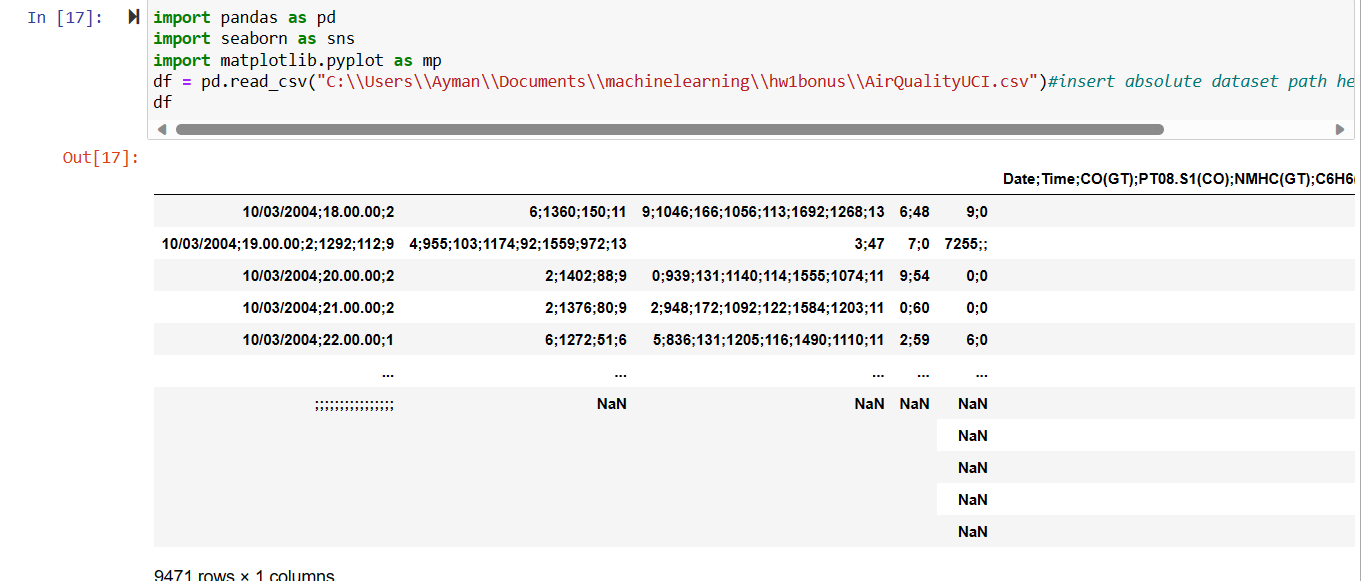
\includegraphics[width=0.5\linewidth]{d.png}
    \caption{Data Frame of Data Set 3}
    \label{fig:enter-label}
\end{figure}
When looking for null values it is apparent that there are null values but using ".describe" does not provide box plot information so it will be best to remove null time stamps from the data set. 
\begin{figure}
    \centering
    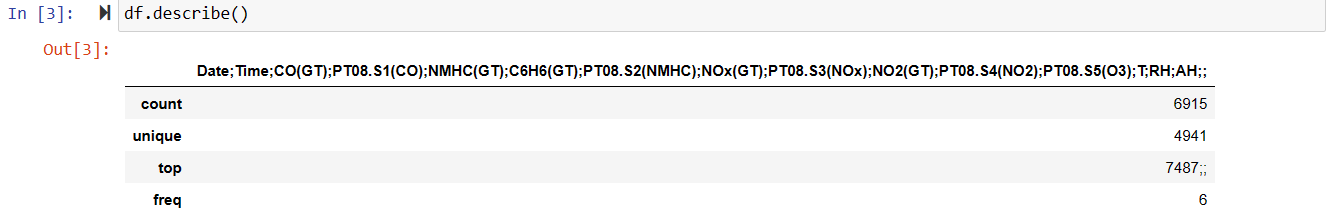
\includegraphics[width=0.5\linewidth]{e.png}
    \caption{Data Frame nulls}
    \label{fig:enter-label}
\end{figure}
Because of how the .csv file uses a mix of semi colons and colons, significant data clean up will be required before further EDA can be conducted.
\begin{figure}
    \centering
    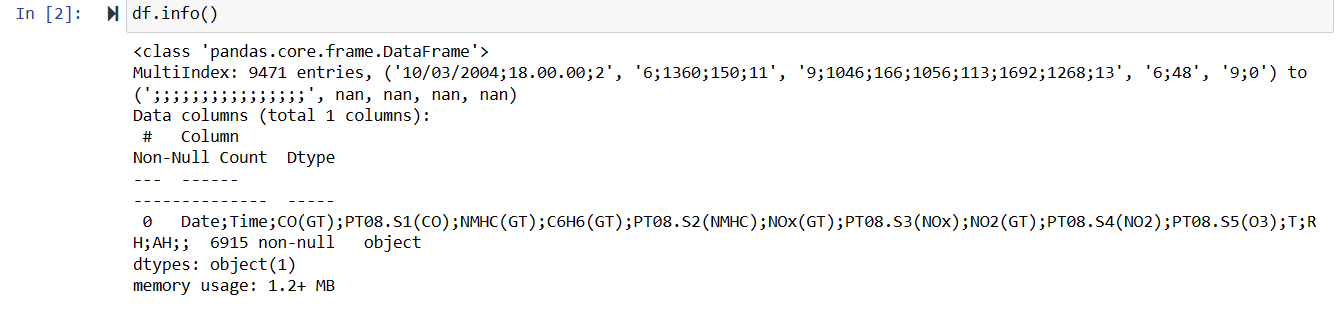
\includegraphics[width=0.5\linewidth]{f.png}
    \caption{Data Frame Info}
    \label{fig:enter-label}
\end{figure}

\section{Data Set 4}
The fourth data set EDA will be performed on is called "ionosphere.csv". 
The data was pulled from the UC Irvine Machine Learning Repository. The data set holds radar information returns about whether they were good or bad. They are separated in categorical attributes with the last attribute being what class of radar it is is. The data frame below provides this information.
\begin{figure}
    \centering
    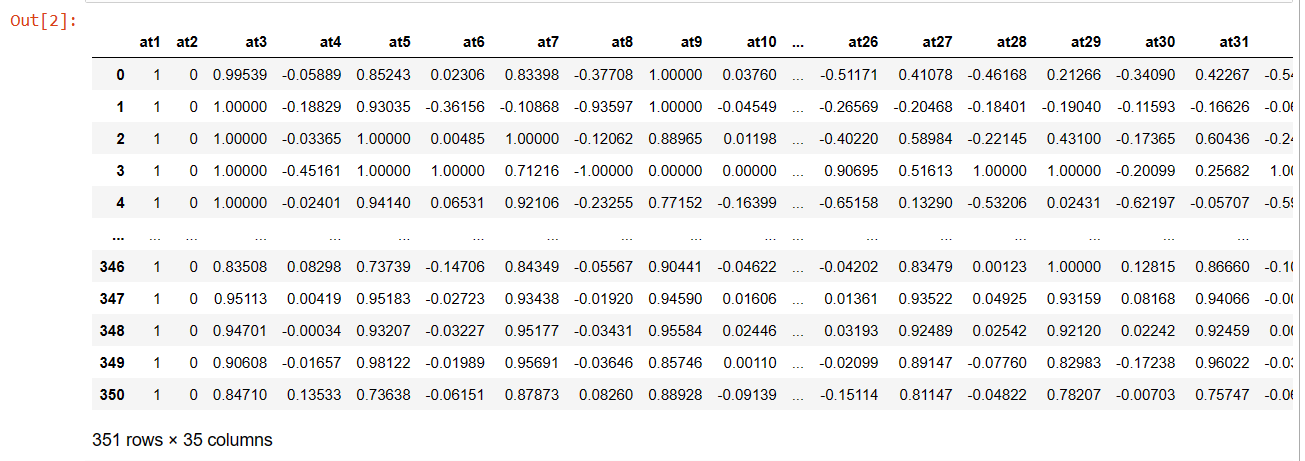
\includegraphics[width=0.5\linewidth]{33.png}
    \caption{Data Frame of Data Set 4}
    \label{fig:enter-label}
\end{figure}
When using info to see what data types are going to be worked with, all entries are floats with the final entry being an object of the radio class.
Luckily, there are no null values in the data set so minimal clean up will be needed. 
\begin{figure}
    \centering
    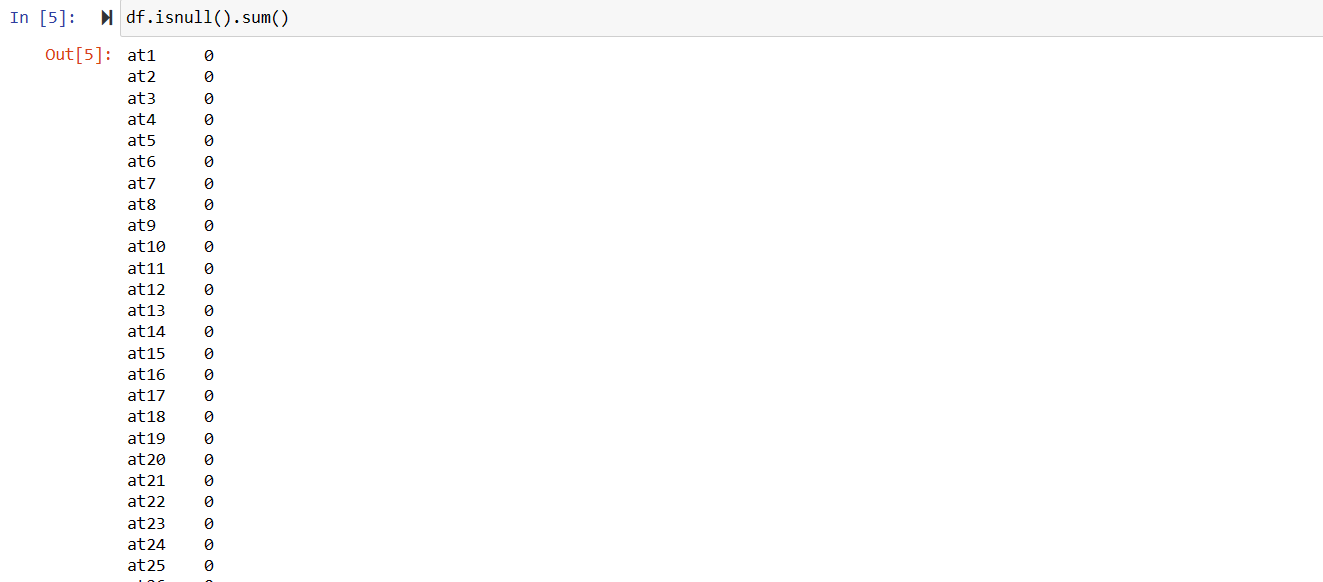
\includegraphics[width=0.5\linewidth]{22.png}
    \caption{Data Frame nulls}
    \label{fig:enter-label}
\end{figure}
When checking for correlation between the radar class and the type of radar return, there is a lack of correlation. Rather, it is the time of day and the positioning of the radar that shows correlation between a good or bad return.
\begin{figure}
    \centering
    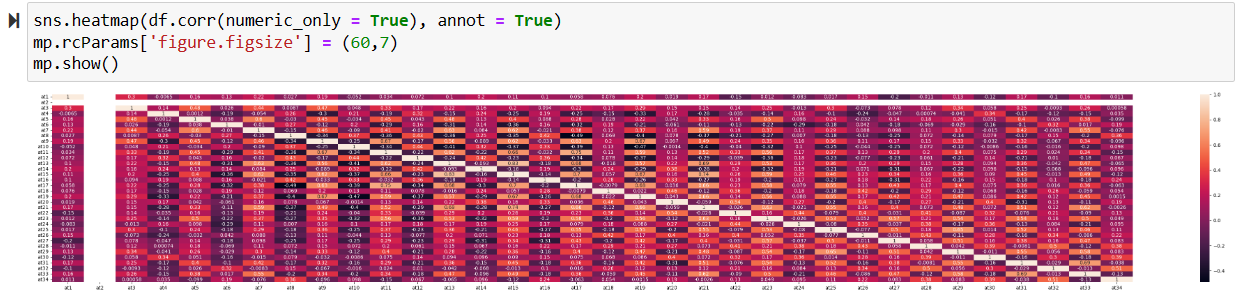
\includegraphics[width=0.5\linewidth]{11.png}
    \caption{Data Frame Heat Map}
    \label{fig:enter-label}
\end{figure}
\section{Data Set 5}
The fifth data set EDA will be performed on is called "Real estate valuation data set.csv". The data was pulled from the UC Irvine Machine Learning Repository. The data set holds information on when a house was sold, its price area, house age, and local features that accompany a house like what stores are near it. The data frame displays such information. 
\begin{figure}
    \centering
    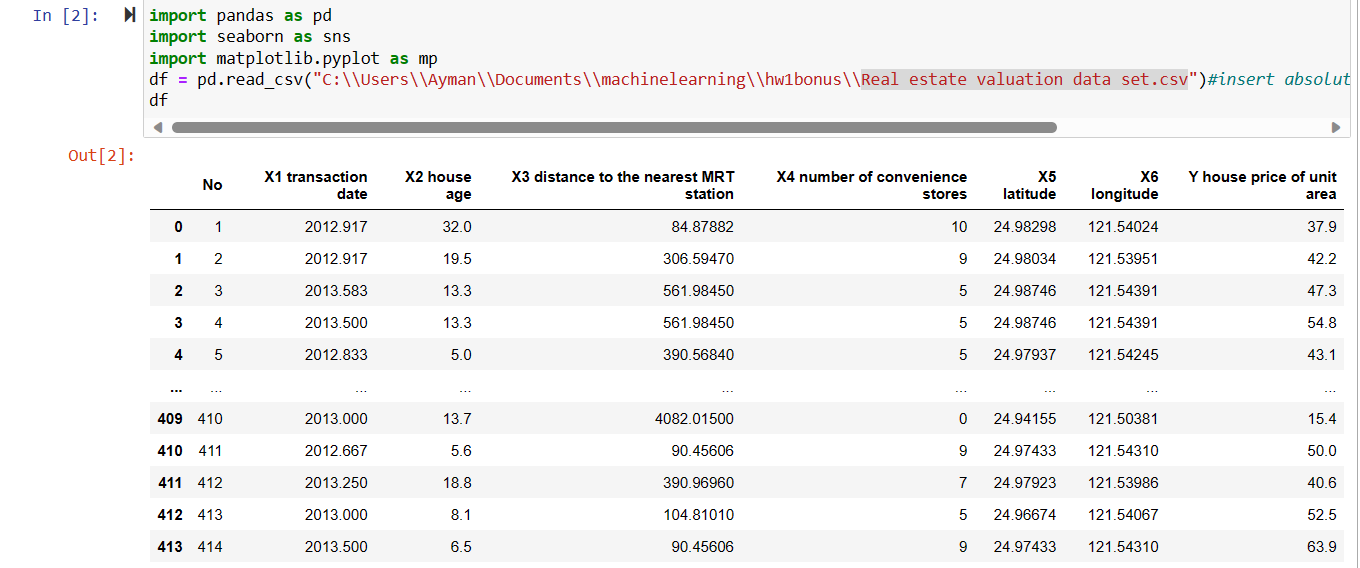
\includegraphics[width=0.5\linewidth]{100.png}
    \caption{Data Frame of Data Set 5}
    \label{fig:enter-label}
\end{figure}
The data types included in the data frame are ints and floats. This will make it easier to conduct calculations and manipulate the data without lossy conversion issues. However the transaction date will need to be converted into an object.
\begin{figure}
    \centering
    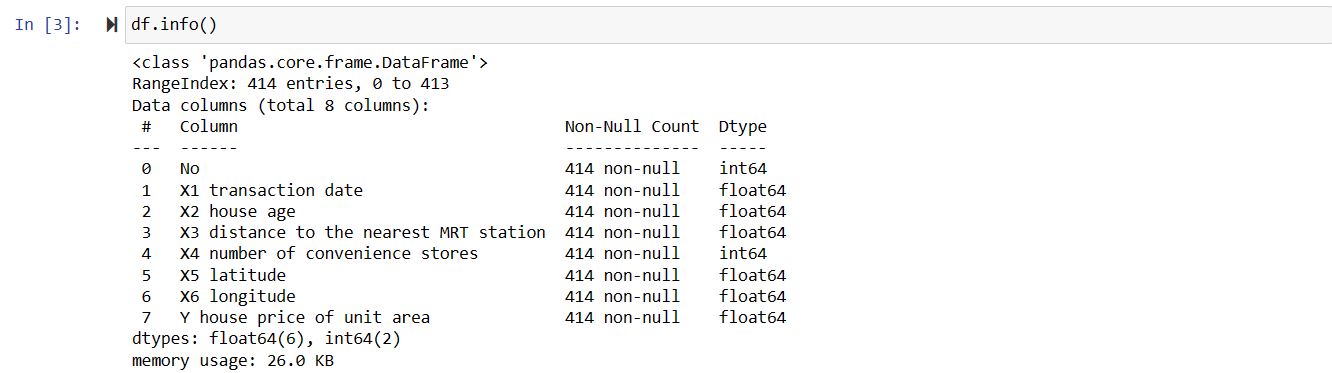
\includegraphics[width=0.5\linewidth]{image.png}
    \caption{Data Frame Info}
    \label{fig:enter-label}
\end{figure}
When describing the data, the average house age sold was 17 years old. The minimum price of unit area was 7.6 while the max was 117.5, a striking range.
\begin{figure}
    \centering
    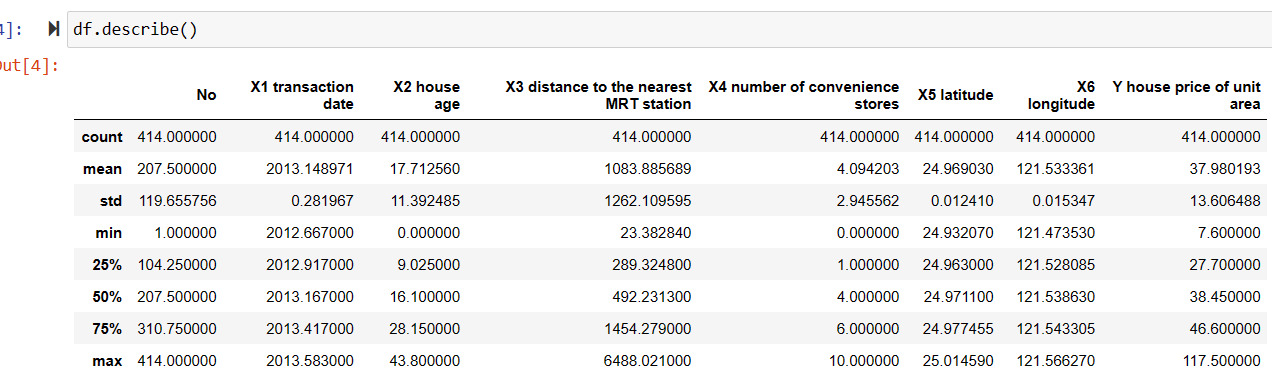
\includegraphics[width=0.5\linewidth]{300.png}
    \caption{Data Frame Describe}
    \label{fig:enter-label}
\end{figure}
After generating a heat map it is difficult to find correlation through what is expected. One would expect that the older the house the cheaper its price, but the correlation did not display that. Rather, the most clear correlation is between price and where that house is located along with the stores near it.
\begin{figure}
    \centering
    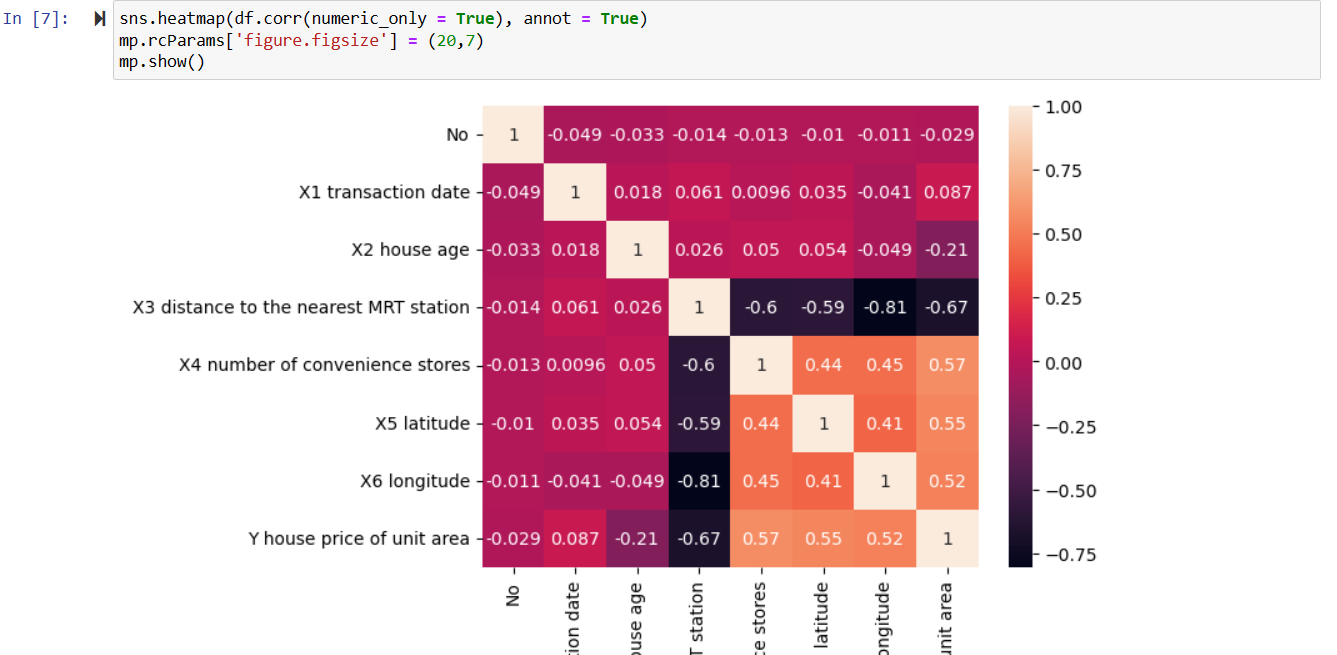
\includegraphics[width=0.5\linewidth]{400.png}
    \caption{Data Frame Heat Map}
    \label{fig:enter-label}
\end{figure}
\end{document}
